\documentclass[class=book, crop=false]{standalone}
\usepackage[subpreambles=true]{standalone}
\RequirePackage{/home/mark/Documents/gradschool/research/thesis/preamble}
\usepackage{import}

\begin{document}

\chapter{Exceptional Cases}
\label{exceptional}
Throughout the chapter, $(G,(U_\alpha)_{\alpha\in \Phi},T)$ will be an RGD system of type $(W,S)$ which also satisfies \eqref{assume}. If we fix a fundamental apartment and fundamental chamber, then we will also assume that $[U_x:U'_x]\ge 2$ where $x$ is the vertex of $C$ of type $s.$ In particular, this implies that $c=m(t,u)\ge 4.$ In the previous chapter we showed that $U_+$ was not finitely generated if either $a$ or $b$ was also at least 4. Therefore, in this chapter we will assume that $a=b=3.$ 

In the previous chapter, one of the key steps to showing that $U_+$ was finitely generated was to show that the region $\D=\alpha_1\cap\alpha_n\cap \beta\cap\beta'$ was infinite, where $\alpha_1,\alpha_n,\beta,\beta'$ are defined as before. We were able to demonstrate an infinite set of chambers contained in $\D$ from specific elements of the Coxeter group $W.$ These proofs did rely on the assumption that $b\ge 4,$ and so we certainly cannot use identical arguments as those that came before. There might be some hope that we can choose the elements of $W$ more carefully to find another infinite family, of chambers, but the following lemma shows this is not possible.


\begin{lemma} 
	\label{lem:infD}
	Let $(W,S)$ be a rank 3 Coxeter system defined by the labels $a,b,c$ as before. Also assume without loss of generality that $a\le b\le c.$ Then the region $\D,$ defined as before, will contain infinitely many chambers if and only if $b\ge 4.$
\end{lemma}
\begin{proof}
	We know by Lemma \ref{lem:infmany} that $\D$ is infinite if $b\ge 4.$ Thus it remains to show that $\D$ is finite if $b=3.$ If $b=3$ then $a=3$ also, and by definition of $a,b,c$ this means $m(s,t)=m(s,u)=3.$ We will also recall the definition of $\D=\alpha_1\cap \alpha_n\cap \beta \cap \beta'$ where
	\begin{align*}
	\alpha_1&=\{D\in \Sigma|d(D,C)<d(D,tC)\}=\{w\in W|\ell(w)<\ell(tw)\}\\
	\alpha_n&=\{D\in \Sigma|d(D,C)<d(D,uC)\}=\{w\in W|\ell(w)<\ell(uw)\}\\
	\beta&=\{D\in \Sigma|d(D,tC)<d(D,tsC)\}=\{w\in W|\ell(tw)<\ell(stw)\}\\
	\beta'&=\{D\in \Sigma|d(D,uC)<d(D,usC)\}=\{w\in W|\ell(uw)<\ell(suw)\}
\end{align*}

Let $w\in W$ and suppose $\ell(w)\ge 2.$ Then we can write $w=s_1s_2w'$ where $\ell(w')=\ell(w)-2.$ If $s_1=t$ then we have
\[
	\ell(tw)=\ell(s_2w')=\ell(w)-1<\ell(w)
\]
which shows $w\not\in \alpha_1$ and thus $w\not\in \D.$ A similar argument shows that $w\not\in \alpha_n$ and thus $w\not\in \D$ if $s_1=u.$

Now we assume $s_1=s$ and so we can also assume $s_2=t,u.$ First let $s_2=t$ so that $w=stw'.$ If $w\not\in \alpha_1$ then $w\not\in \D$ and so we will suppose $w\in\alpha_1.$ Now we can see
\[
	\ell(stw)=\ell(ststw')=\ell(sstsw')=\ell(tsw')\le \ell(w')+2=\ell(w)<\ell(tw)
\]
and thus $w\not\in \D.$ A similar argument shows that $w\not\in \D$ if $s_2=u.$

We have shown that if $\ell(w)\ge 2$ then $w\not\in \D$ and thus $\D$ must be finite as desired. In fact, if $a=b=3$ then we can check relatively easily that $\D=\{C,sC\}$ which proves the desired result.
\end{proof}

The previous lemma shows that finding chambers of $\D$ is not simply a matter of more clever choices of $W.$ We will therefore have to find a new approach to the remaining cases. Before tackling these cases, we will first enumerate what remains to be shown.

With the assumptions of this chapter we know $(W,S)$ is a Coxeter system with $S=\{s,t,u\}.$ We assume that $m(s,t)=m(s,u)=3$ so that $\lk(v')$ will not be one of the exceptional Moufang polygons if $v'$ has type $u$ or $t.$ We want to assume that the building $\Delta$ does have an exceptional link as otherwise there is nothing new two show, so we will assume that there is a vertex $v,$ of type $s,$ with link corresponding to one of the 4 exceptional Moufang polygons. This implies that every vertex of type $s$ will have an exceptional link, and we let $x$ be the vertex of $C$ of type $s$ for some choice of fundamental chamber $C$ and fundamental apartment $\Sigma.$

Citing Lemma \ref{lem:index} again we see that $\lk(x)$ must be the Moufang Polygon associated to one of the groups $C_2(2),G_2(2),G_2(3),{}^2F_4(2).$ According to private communication with Bernhard M\"{u}hlherr the case where $\lk(x)$ is associated to ${}^2F_4(2)$ is impossible and so we have just the 3 possibilities to consider. We will handle these in separate sections.

\section{Case: $\lk(x)$ associated to the group $G_2(2)$}
Assume that $(G,(U_\alpha)_{\alpha\in \Phi},T)$ is an RGD system of type $(W,S)$ as in the setup. Choose a fundamental apartment and chamber $\Sigma$ and $C$ of the associated building $\Delta,$ and assume that $\lk(x)$ is the building associated to $G_2(2)$ where $x$ is the vertex of $C$ of type $s.$ Notably this implies that $m(t,u)=6.$

We saw in the previous chapter that a vertex contained in $\D$ was a sufficient condition to construct a corresponding map $\tilde{\phi_v}.$ However, it is not a necessary condition, and we will see in this section we can relax a few conditions to still construct $\tilde{\phi_v}$ for infinitely many vertices. Our first step is to make some general observations about this case and then prove a statement similar to Lemma \ref{lem:existence}.

We still have the presentation of $U_+$ as in Lemma \ref{lem:upres} and so extending $\phi_v$ is still a matter of checking the commutator relations in $U_+.$ We want to extend the map in the same way by defining $\tilde{\phi}_v$ by
\[
	\tilde{\phi}_v(u)=\begin{cases}\phi_v(u)&v\in \partial\alpha\text{ and }u\in U_\alpha\\
	1&\text{otherwise}\end{cases}
\]
Using the properties outlined in Chapter 4 we can prove the following Lemma.

\begin{lemma} 
	\label{lem:336f2ex}
	Let $v$ be a vertex of $\Sigma$ of type $s,$ meaning $|\st(v)|=12.$ Assume $\gamma_1,\dots,\gamma_6$ is a standard ordering of the positive roots through $v$ such that $U_{\gamma_2}\subset \ker \phi_v.$ If $\gamma_3,\gamma_4,$ and $\gamma_5$ are simple at all other vertices they meet, then $\tilde{\phi_v}$ as defined in Lemma \ref{lem:existence} exists.
\end{lemma}
\begin{proof}
	First we mention that it is always possible to choose a standard ordering of $\gamma_1,\dots,\gamma_6$ such that $U_{\gamma_2}\subset \ker\phi_v$ by Lemma \ref{lem:normal} and Corollary \ref{cor:phiv}.

	To check $\tilde{\phi_v}$ is well defined is a matter of checking the relations of $U_+$ are satisfied by the images under $\tilde{\phi_v}.$ The proof is similar to that for Lemma \ref{lem:existence}. In fact, the identical argument shows that relations in $U_\alpha$ and commutator relations with nested roots will again be satisfied. Thus it remains to check commutator relations between roots with intersecting walls.

	Suppose $\alpha$ and $\beta$ are any two positive roots with $y=\partial\alpha\cap \partial\beta.$ Then there is a relation in $U_+$ of the form $[u,u']=w$ where $u\in U_\alpha, u'\in U_\beta,$ and $w\in U_{(\alpha,\beta)}.$ Since $[u_\alpha,u_\beta]$ must be mapped to the identity then we just need to check that $w$ is also mapped to the identity. If $y=v$ then $u_\alpha,u_\beta,w$ all lie in $U_v$ and $\tilde{\phi_v}(w)=\phi_v(w)$ which must be the identity because $\phi_v$ is a well defined homomorphism.

	Now suppose $y\neq v.$ Let $\delta_1,\dots,\delta_n$ be the positive roots through $y,$ with a standard labeling, and assume that $\alpha=\delta_i$ and $\beta=\delta_j$ with $i<j.$ There is at most one positive root whose wall can pass through both $v$ and $y,$ call it $\delta_k$ if it exists. If $\delta_k$ does not exist, then no positive roots through $y$ pass through $v$ and so $\tilde{\phi_v}(u_{\delta_m})=1$ for all $m.$ Thus $\tilde{\phi_v}(w)=1$ as desired.

	Now suppose $\delta_k$ does exist and $\delta_k=\gamma_r$ for $r\in \{1,2,6\}.$ Then we know $\tilde{\phi_v}(U_{\delta_m})=\{1\}$ for all  $m\neq k$ and $\tilde{\phi_v}(U_{\delta_k})=\tilde{\phi_v}(U_{\gamma_r})=\phi_v(U_{\gamma_r})=\{1\}$ by the construction of $\phi_v.$ Thus $\tilde{\phi_v}(U_{\delta_m})=\{1\}$ for all $m$ and so $\tilde{\phi_v}(w)=\{1\}$ as well.

	Now suppose $\delta_k$ does exist and $\delta_k=\gamma_r$ for $r\in \{3,4,5\}.$ Then by assumption, $\delta_k$ is simple at $y$ and thus $k=1,n.$ Thus $\tilde{\phi_v}(U_{\delta_m})=\{1\}$ for all $2\le m\le n-1.$ But $w$ is a word in $U_{(\alpha,\beta)}\subset U_{(\delta_2,\delta_{n-1})}$ and thus $\tilde{\phi_v}(w)=1$ again, which gives the result.
\end{proof}

It is worth noting that the hypotheses of this Lemma are weaker than those of Lemma \ref{lem:existence}, and so we have a hope of constructing more $\tilde{\phi_v}$ than the theory of the previous chapter would allow us to. However, many of the ideas will still be similar and the proofs in this section will run parallel to those in the previous chapter.

Now recall that $x$ is the vertex of $C$ of type $s$ so that $[U_x:U'_x]=2.$ Let $\alpha_1,\dots,\alpha_6$ be a standard labeling of the positive roots through $x$ such that $\phi_x(U_{\alpha_2})=\{1\},$ which we may do by Lemma \ref{lem:normal} and Corollary \ref{cor:phiv}. As in the previous chapter we define roots
	\begin{align*}
		\alpha_1&=\{D\in \Sigma|d(D,C)<d(D,tC)\}=\{w\in W|\ell(w)<\ell(tw)\}\\
		\alpha_6&=\{D\in \Sigma|d(D,C)<d(D,uC)\}=\{w\in W|\ell(w)<\ell(uw)\}\\
		\beta'&=\{D\in \Sigma|d(D,uC)<d(D,usC)\}=\{w\in W|\ell(uw)<\ell(suw)\}
	\end{align*}
	Now define $\D'=\alpha_1\cap \alpha_6\cap \beta'.$ We will now prove a result similar to Lemma \ref{lem:containD} in the current context.


	\begin{figure}
		\begin{center}
			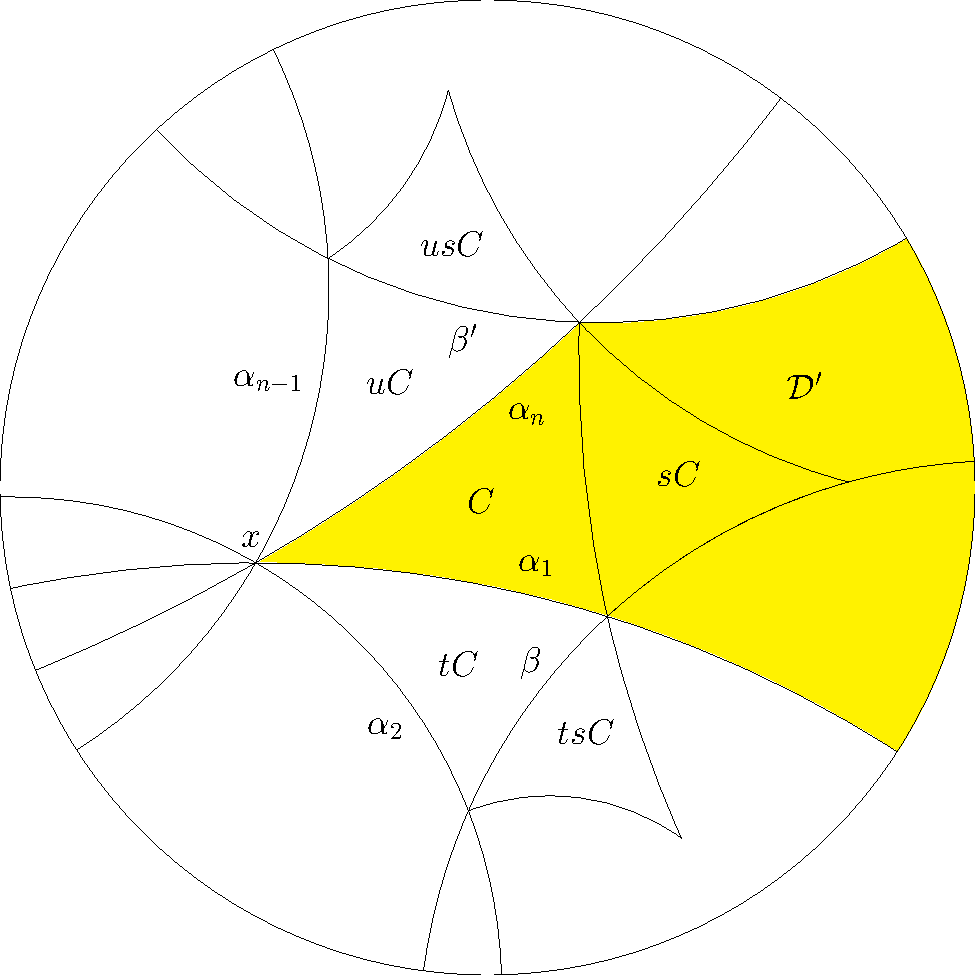
\includegraphics[width=3.5 in]{diagrams/defineDprime.pdf}
		\end{center}
		\caption{The roots $\alpha_1,\alpha_n,\beta'$ with the region $\D'$ in yellow.}
		\label{fig:defineDprime}
	\end{figure}

\begin{lemma}
	\label{lem:336f2D}
	Let $x$ be the vertex of $C$ of type $s$ so that $|\st(x)|=12.$ Let $\alpha_1,\dots,\alpha_6$ be the positive roots at $x$ with a standard ordering. Also assume that $\phi_x(U_{\gamma_2})=1.$ Suppose $\gamma=\alpha_i$ for $i\in \{3,4,5\}.$ If $\delta$ is any positive root with $\partial\gamma\cap \partial\delta\neq \emptyset$ then $\D'=\alpha_1\cap \alpha_6\cap \beta'\subset \gamma\cap \delta$ where 
	\begin{align*}
		\alpha_1&=\{D\in \Sigma|d(D,C)<d(D,tC)\}=\{w\in W|\ell(w)<\ell(tw)\}\\
		\alpha_6&=\{D\in \Sigma|d(D,C)<d(D,uC)\}=\{w\in W|\ell(w)<\ell(uw)\}\\
		\beta'&=\{D\in \Sigma|d(D,uC)<d(D,usC)\}=\{w\in W|\ell(uw)<\ell(suw)\}
	\end{align*}
	as in the previous chapter.
\end{lemma}
\begin{proof}
	Since $\gamma$ is a positive root at $x,$ and $\alpha_1,\alpha_6$ are the simple roots at $x,$ we know that $\D'\subset \alpha_1\cap \alpha_6\subset \gamma$ and thus it will suffice to show that $\D'\subset \delta.$

	Let $y=\partial\gamma \cap \partial \delta.$ If $y=x$ then $\delta$ is also a root which passes through $x$ and so $\delta=\alpha_j$ for some $j\neq i.$ Then as before we get $\alpha_1\cap \alpha_6\subset \alpha_j=\delta$ and thus $\mathcal{D}'\subset \delta$ so that $\mathcal{D}'\subset \gamma\cap \delta$ as desired.

	Now suppose that $\partial \gamma\cap \partial \delta=y\neq x.$ From the local geometry of $\Sigma$ around $x$ we can see the following facts. For any $\alpha_i$ with $2\le i\le n-1$ we know that $\partial\alpha_i\cap \alpha_1\cap \alpha_6=\{x\}$ and $\partial\alpha_i\subset \alpha_1\cup\alpha_6.$ Thus the point $y$ will lie in exactly one of $\alpha_1$ or $\alpha_6.$

	First suppose that $y\in \alpha_1$ so that $y\not\in \alpha_6.$ If $\partial\alpha_6\cap \partial\delta=\emptyset$ then there are exactly 3 possibilities. Either $\alpha_6\subset \delta,$ $\delta\subset\alpha_6,$ or $-\delta\subset \alpha_6.$ But the last two possibilities would contradict our assumption that $y\not\in \alpha_6$ and thus we get $\alpha_6\subset \delta$ and thus $\D'\subset \alpha_6\subset \gamma\cap\delta$ as desired.

	Alternatively, assume that $\partial\alpha_6\cap \partial\delta=y'.$ Then the points $x,y,y'$ will form a triangle with sides on walls of $\Sigma.$ Then by the triangle condition, these three vertices must form a chamber, call it $E.$ The points $x,y$ lie on $\partial\gamma=\partial\alpha_i$ and the points $x,y'$ lie on $\partial\alpha_6.$ Since $y$ and $y'$ are adjacent this means that either $\gamma=\alpha_5$ or $\gamma=\alpha_1.$ The latter is a contradiction of our assumptions and thus $\gamma=\alpha_5.$ We know that $y$ and $y'$ are adjacent and $y\in \alpha_1.$ Since neither $y$ or $y'$ lies on $\partial\alpha_1$ this means that $y'\in \alpha_1$ as well.

	We know that $E$ is a chamber in $\st(x)$ with a side on $\partial \alpha_6$ and $\partial\alpha_5.$ let $D=tC$ and $D'$ be the chamber opposite $D$ in $\st(x).$ Then either $E=D$ or $E=D'.$ By definition, $\alpha_6$ is the only wall separating $C$ and $tC$ which means $D=tC\in \alpha_1.$ If $E=D'$ then $D'\in \alpha_1$ since $x,y,y'$ all lie in $\alpha_1.$ But this is a contradiction as $\alpha_1$ cannot contain two opposite chambers in $\st(x).$ Thus $E=D=tC$ and $\delta=\beta$ by definition. Thus $\D'\subset \beta=\delta$ and $\D'\subset \gamma\cap \delta$ as desired.

	If we assume instead that $y\in\alpha_1$ so that $y\not\in \alpha_6$ then we have the same two possibilities. If $\partial \alpha_6\cap \partial \delta=\emptyset$ then by similar arguments we get $\D'\subset \alpha_6\subset \delta$ and thus $\D'\subset \gamma\cap \delta$ as desired. If $\partial \alpha_6\cap \partial\delta=y'$ then the vertices $x,y,y'$ form a chamber with $y'$ on $\alpha_6.$ Again, by similar arguments as before, this would imply that $\gamma=\alpha_2$ or $\alpha_6,$ both of which are impossible.

	Therefore, regardless of case we have $\D'\subset \gamma\cap \delta$ as desired.
	

\end{proof}
%             I don't think I need this proof any more
%
%The proofs in the previous chapter relied heavily on facts about simple roots, and to aid these proofs we had Lemma \ref{preservesimple} which shows the $W$ action on $\Sigma$ preserves simplicity under certain condidtions. Now that we are dealing more than just simple roots we need to extend this lemma to the current context.
%
%\begin{lemma}
%	\label{preservemapto1}
%	Suppose $v$ is a vertex of $\Sigma$ of type $s$ so that $U'_v\neq U_v,$ and $w\in W$ such that $w\gamma$ is a positive root at $wv$ for all positive roots $\gamma$ at $v.$ If $\delta$ is a positive root at $v$ such that $\phi_v(u_\delta)=1$ then $\phi_{wv}(u_{w\delta})=1$ as well.
%\end{lemma}
%\begin{proof}
%	We know from the theory of Moufang twin buildings that there is some $\tilde{w}\in \mathrm{Aut}(\Delta)$ such that $\tilde{w}U_\alpha\tilde{w}^{-1}=U_{w\alpha}$ for all roots $\alpha\in \Phi.$ Let $\psi_w:\G\to \G$ be the conjugation isomorphism defined by $\tilde{w}.$ For any positive root $\gamma$ at $v,$ we know $w\gamma$ is positive at $wv$ by assumption, and thus $\psi_w(u_\gamma)=u_{w\gamma}\in U_{w\gamma}.$ Thus the map $\psi_w$ restricts to a map from $U_v$ to $U_{wv}$ which is necessarily injective. Now suppose $\gamma'$ is a positive root at $wv.$ There are only finitely many roots at $v$ and $wv,$ and since $w$ sends positive roots to positive roots, it must also send negative roots to negative roots. Thus $w^{-1}$ must also send positive roots at $wv$ to positive roots at $v.$ Thus $w^{-1}\gamma'$ is a positive root at $v.$ Thus $\psi_w(u_{w^{-1}\gamma'})=\gamma'$ which means $\psi_w:U_v\to U_{wv}$ is surjective and thus an isomorphism.
%
%	Now consider the map $f=\phi_{wv}\psi_w:U_v\to K.$ We know $\psi_w$ is an isomorphism, and $\phi_{wv}$ is surjective and thus $f$ is surjective. By Lemma \ref{preservesimple} we know that if $\gamma$ is simple at $wv$ then $w^{-1}\gamma$ is simple at $v$ and $f(u_{w^{-1}\gamma})=\phi_{wv}(\gamma)=1$ by the definition of $\phi_{wv}.$ Thus if $U_1,U_6$ are the simple roots at $v$ then $U_1,U_6\le \ker f.$ Thus $\ker f$ is a normal subgroup of $U_v$ containing $U_1$ and $U_6$ so $\ker f=\ker \phi_v$ by Lemma \ref{uniquephiv}.
%
%	Since $\psi_w$ is an isomorphism we know $\ker \phi_{wv}=\psi_w(\ker f)=\psi_w(\ker \phi_{v})$ and thus if $u_\delta\in \ker \phi_v$ then $\psi_w(u_\delta)=u_{w\delta}\in \ker \phi_{wv}$ which gives the desired result.
%\end{proof}
%
We now have a condition for $\tilde{\phi}_v$ to exist which we can check and so it remains to find potential candidates to use at $v.$ We know by Lemma \ref{lem:resporder} that $\phi_{v}$ will exist for all vertices $v$ of type $s.$ We will us a strategy similar to that of the previous chapter which relies on the definition of $\D'$ to show $\tilde{\phi}_v$ exists for certain $v.$ To this end we now prove the analogue of Lemma \ref{lem:Dexists}.

\begin{lemma} 
	\label{lem:336f2Dex}
 Let $x$ be the vertex of $C$ of type $s$ and suppose that $v$ is any vertex in $\D'=\alpha_1\cap \alpha_6\cap \beta$ of type $s.$ Then there is a $w\in W$ such that $w^{-1}x=v$ and $\tilde{\phi}_{wx}$ exists.
\end{lemma}
\begin{proof}
	The proof is nearly identical to that of Lemma \ref{lem:Dexists}. Let $D=\mathrm{Proj}_{v}(C)$ and define $w$ so that $D=w^{-1}C.$ By definition, $v$ is a vertex of $D$ of type $s$ and $w^{-1}x$ is also a vertex of $D$ of type $s$ and thus $w^{-1}x=v.$ The claim is that this $w$ will satisfy the desired properties. First we mention that $wx$ is also a vertex of $\Sigma$ of type $s$ and thus $[U_{wx}:U'_{wx}]\ge 2$ and $\phi_{wx}$ exists by Corollary \ref{cor:respectphiv}. 
	
	Again, the definition of projections means that $D$ is the closest vertex to $C$ which has a vertex of $w^{-1}x.$ Since $\D'$ is convex, and $w^{-1}x$ and $C$ both lie in $\D',$ we also know that $D=\mathrm{Proj}_{w^{-1}x}(C)$ lies in $\D'$ as well. By a similar argument we know that $\mathrm{Proj}_{x}(D)$ must lie in $\D'\subset \alpha_1\cap \alpha_6$ and thus $\mathrm{Proj}_{x}(D)=C.$ Now define $E=wC$ and note that the action of $W$ respects projections and thus we have
	\[
		E=wC=\mathrm{Proj}_{wx}{wD}=\mathrm{Proj}_{wx}{C} \qquad C=wD=\mathrm{Proj}_{w(w^{-1}x)}{wC}=\mathrm{Proj}_{x}{E}
	\]
In particular, a root through $wx$ is positive if and only if it contains $E.$

Our goal is to apply Lemma \ref{lem:336f2ex} at the vertex $wx.$ Let $\gamma_1,\dots,\gamma_6$ be a standard labeling of the positive roots through $wx$ such that $U_{\gamma_2}\subset \ker \phi_{wx}.$ We need to check that if $y\neq wx$ is on $\partial\gamma_i$ for $i\in \{3,4,5\}$ then $\gamma_i$ is simple at $y.$ First we will show that $w^{-1}$ sends positive roots at $wx$ to positive roots at $x.$ Suppose $\gamma$ is any positive root at $wx.$ Then we know that $E\in \gamma$ and thus $C=w^{-1}E\in w^{-1}\gamma$ so that $w^{-1}\gamma$ is positive, and thus $w^{-1}$ sends positive roots at $wx$ to positive roots at $x.$

If we apply Lemma \ref{lem:resporder} then we know that $w^{-1}\gamma_1=\alpha_1,\dots,w^{-1}\gamma=\alpha_6$ is a standard labeling of the of the positive roots at $x.$ If we apply this isomorphism given by Corollary \ref{cor:respectphiv} then we know that $U_{w^{-1}\gamma_2}=U_{\alpha_2}\subset \ker \phi_x$ since $U_{\gamma_2}\subset \ker \phi_{wx}.$ 

Now we fix $i\in \{3,4,5\}$ and we need to check $\gamma_i$ is simple at all vertices $y\neq v$ on $\partial\gamma_i.$ If we apply $w^{-1}$ we get that $w^{-1}y\neq x$ is a vertex on $\partial \alpha_i.$ Thus by Lemma \ref{lem:xpos} we know that $\alpha_i$ is simple at $w^{-1}y.$ Now suppose that $\delta$ is any positive root at $w^{-1}y.$ Recall that $D\in \D'$ and we can apply Lemma \ref{lem:336f2D} to see that $\D'\subset \delta$ so that $D\in \delta.$ If we apply $w$ we get $C=wD\in w\delta$ so that $w\delta$ is a positive root through $w(w^{-1}y)=y.$ Thus $w$ sends positive roots at $w^{-1}y$ to positive roots at $y.$ We can apply Lemma \ref{lem:resporder} again to say that $w$ sends the simple roots at $w^{-1}y$ to the simple roots at $y.$ Since $\alpha_i$ is simple at $w^{-1}y$ we know that $w\alpha_i=\gamma_i$ is simple at $y$ as desired. We now for all positive roots $\gamma_i$ for $i\in \{3,4,5\}$ at $wx$ that $\gamma_i$ is simple at all other vertices, and thus we can apply Lemma \ref{lem:336f2ex} to say that $\tilde{\phi}_{wx}$ exists as desired.


\end{proof}

As in the previous chapter, we now have a potentially large class of vertices for which $\tilde{\phi}_v$ exists, but we still must show there are infinitely many, and that they do not lie on finitely many walls. The approach will be similar as in the previous chapter, and recall in our current setup that $m(s,t)=m(s,u)=3$ and $m(t,u)=6.$

\begin{lemma}
	\label{lem:336f2inf}
	Let $w_k=(uts)^k$ for all $k\ge 0$ and let $x$ be the vertex of $C$ of type $s.$ Then the vertices $(w_k)^{-1}x$ are all distinct, and they all lie in $\D'=\alpha_1\cap \alpha_6\cap\beta$ as defined previously.
\end{lemma}
\begin{proof}
	The proof will be similar to that of Lemma \ref{lem:infmany}. First note that $(w_k)^{-1}=(stu)^k$ for all $k.$ Since $(w_k)^{-1}x$ is a vertex of $(w_k)^{-1}C,$ it will suffice to show that $(w_k)^{-1}C$ is a chamber of $\D'.$ Now we may use the identification of chambers with the elements of $W,$ and work with the length function and M-Operations. There are certainly no M-Operations possible in $w_k^{-1}$ so we have $\ell(w_k^{-1})=3k.$ There are also no M-Operations possible in $uw_k^{-1}=u(stustu\cdots)$ which means $\ell(uw_k^{-1})=3k+1$ so that $w_k^{-1}\in \alpha_6.$ Some computation also shows that
	\begin{align*}
		tw_k^{-1}&=t(stustus\cdots)\\
			 &=(tst)(ustus\cdots)\\
			 &=(sts)(ustus\cdots)\\
			 &=(st)(sus)(tus\cdots)\\
			 &=(st)(usu)(tus\cdots)\\
			 &=(st)(us)(utus\cdots)
	\end{align*}
	which exhausts all of the possible M-Operations in $tw_k^{-1}.$ Since no operations of type 1 were performed, we have $\ell(tw_k^{-1})=3k+1$ so that $tw_k^{-1}\in \alpha_1$ as well.

	Finally, we check that
	\begin{align*}
		suw_k^{-1}&=su(stustus\cdots)\\
			  &=(sus)(tustus\cdots)\\
			  &=(usu)(tustus\cdots)\\
			  &=(us)(utustus\cdots)\\
	\end{align*}
	which shows by the same logic that $\ell(suw_k^{-1})=3k+2$ and $suw_k^{-1}\in \beta'.$ Therefore, $w_k^{-1}x$ is a vertex in $\alpha_1\cap \alpha_6\cap \beta'$ for all $k\ge 0$ as desired.
\end{proof}

The previous proof shows that the vertices $w_k^{-1}x$ are all distinct and lie in $\D',$ which means each one will give rise to a $\tilde{\phi}_wx$ for some $w.$ If we check the proof of Lemma \ref{lem:336f2Dex} then we can verify that $w_k$ will satisfy the properties of the desired $w,$ and thus $\tilde{\phi}_{w_kx}$ will exist for all $k.$ The last major step is to show that these $w_kx$ cannot all lie on finitely many walls.

\begin{lemma}
	\label{lem:336f2walls}
	Let $x$ be the vertex of $C$ of type $s$ and let $w_k=(uts)^k$ for all $k\ge 0.$ Any wall of $\Sigma$ can contain only finitely many $w_kx.$
\end{lemma}
\begin{proof}
	The proof is nearly identical to that of Lemma \ref{lem:samewall}. Suppose that $w_mx$ and $w_nx$ lie on the same wall for $m>n\ge 0.$ Then we also have $w_{n-m}x$ and $x$ lie on the same wall. The walls passing through $x$ are exactly the walls $\partial\alpha_1,\dots,\partial\alpha_6.$ But $w_{n-m}=w_k^{-1}$ for $k=m-n\ge 1$ so $w_{n-m}x$ lies in $\D'\subset \alpha_1\cap \alpha_6.$ As mentioned before, $\partial\alpha_i\cap \alpha_1\cap \alpha_6=\{x\}$ for $2\le i\le 5$ and thus $w_{n-m}x$ will lie on $\partial\alpha_1$ or $\partial\alpha_6.$ These walls are the fixed points of the reflections $t$ and $u$ respectively, so we have either $tw_{n-m}x=w_{n-m}x$ or $uw_{n-m}x=w_{n-m}x.$ This would mean that one of $w_{n-m}^{-1}tw_{n-m}$ or $w_{n-m}^{-1}uw_{n-m}$ lie in $\mathrm{stab}_W(x)=\langle u,t\rangle.$ This can be checked using M-Operations and we see that
	\begin{align*}
		w_{n-m}^{-1}tw_{n-m}&=(\cdots utsutsuts)t(stustustu\cdots)\\
		&=(\cdots utsutsut)(sts)(tustustu\cdots)\\
		&=(\cdots utsutsut)(tst)(tustustu\cdots)\\
		&=(\cdots utsutsu)s(ustustu\cdots)\\
		&=(\cdots utsut)(susus)(tustu\cdots)\\
		&=(\cdots utsut)(u)(tustu\cdots)\\
		&=(\cdots uts)(ututu)(stu\cdots)
	\end{align*}
	and no further M-operations are possible. While we were able to do some reductions in length, we have shown that $w_{n-m}^{-1}tw_{n-m}$ can only be contained in $\langle u,t\rangle$ if $m-n\le 2.$ By a similar computation we can see that
	\begin{align*}
		w_{n-m}^{-1}uw_{n-m}&=(\cdots utsutsuts)u(stustustu\cdots)\\
		&=(\cdots utsutsut)(sus)(tustustu\cdots)\\
		&=(\cdots utsutsut)(usu)(tustustu\cdots)\\
		&=(\cdots utsuts)(utu)s(utu)(stustu\cdots)
	\end{align*}
	and any further M-operations are impossible. In either case we have shown that $w_mx$ and $w_nx$ can only lie on the same wall if $|m-n|\le 2$ and thus only finitely many $w_k x$ can lie on any wall as desired.
\end{proof}

Now we are ready to prove the main result of the section, which extends the result of Theorem \ref{thm:notfg} to this new case.
\begin{theorem}
	\label{thm:336f2notfg}
	Let $(G,(U_\alpha)_{\alpha\in Phi},T)$ be an RGD system of type $(W,S)$ with assumptions as in $\eqref{assume}.$ Suppose that $a=m(s,t)=b=m(s,t)=3.$ Also suppose that $\lk(x)$ is the Moufang polygon associated to the group $G_2(2),$ where $x$ is the vertex of the fundamental chamber $C$ of type $s.$ Then $U_+$ is not finitely generated.
\end{theorem}
\begin{proof}
	Suppose that $U_+$ is finitely generated. Then there is some finite set of roots $\beta_1,\dots,\beta_m$ such that $U_+=\langle U_{\beta_i}|1\le i\le m\rangle.$ Let $w_k=(uts)^k$ for all $k\ge 0.$ Now only finitely many of the vertices $w_kx$ lie on the same wall and thus we can choose $k$ so that $v=w_kx$ does not lie on $\partial \beta_i$ for any $i.$ By Lemma \ref{lem:336f2inf} we know that $\tilde{\phi}_v$ exists, and by definition it is a surjective map from $U_+\to H.$ However, we can also see by definition that $\tilde{\phi}_v(U_{\beta_i})=1$ for all $i,$ since none of these walls meet $v.$ But this means $\tilde{\phi}_v$ sends all of the generators of $U_+$ to the identity and thus it must be the trivial map which is a contradiction. Thus $U_+$ is not finitely generated as desired.
\end{proof}

In keeping with the theme of copying Chapter \ref{ch:general} nearly verbatim, we also get the following Corollary
\begin{cor}
	If $(G,(U_\alpha)_{\alpha\in Phi},T)$ as in Theorem \ref{thm:336f2notfg}, then $(U_+)_{\text{ab}}$ is not finitely generated.
\end{cor}
\begin{proof}
	The proof is identical to that of Corollary \ref{cor:abnotfg}.
\end{proof}

There are two more cases to consider and they will be the topic of the next section.

\section{Case: $\lk(x)$ associated to the group $C_2(2)$ or $G_2(3)$}
The two remaining cases to consider are as follows. $(G,(U_\alpha)_{\alpha\in \Phi},T)$ is an RGD system of type $(W,S)$ satisfying \eqref{assume}. We also assume that $x$ is the vertex of the fundamental chamber $C$ of type $s$ and $\lk(x)$ is the Moufang polygon associated to the group $C_2(2)$ or $G_2(3).$ Finally we assume that $a=m(s,t)=b=m(s,u)=3.$

In the previous section we were able to modify the strategy of Chapter \ref{ch:general} to see that $U_+$ was not finitely generated. No amount of modification to that strategy will work in the current context as we will show that in these cases, the group $U_+$ will be finitely generated. We will do this by defining a filtration of $U_+$ with nice finiteness properties.

We will say that a chamber $D$ borders a root $\alpha$ if a panel of $\D$ lies on the wall $\partial \alpha.$ For any positive root $\alpha\in \Phi$ this allows us to define $d(\alpha,C)$ to be $\min\{d(D,C)|D\text{ borders }\alpha.$ If $d(\alpha,C)=n$ then we know there is some chamber $D$ such that $D$ borders $\alpha$ and $d(D,C)=n.$ Furthermore, we know that $D$ must be a chamber of $\alpha,$ as otherwise there would be a chamber $D'$ adjacent to $D$ across $\partial\alpha$ with $d(D',C)<d(D,C).$ 

	We can define subgroups $U_k$ for all $k\ge 1$ where $U_k=\langle U_\gamma|d(\gamma,C)\le k,\gamma\in \Phi_+\rangle\le U_+.$ From the definition we have $U_1\subset U_2\subset \cdots$ and we also can see that $U_+=\cup_{k\ge 1}U_k$ since any root of $\Phi_+$ will be some finite distance away from $C.$ Since chambers of $\Sigma$ correspond to elements of $W,$ for any $k\ge 1$ there are only finitely many chambers at distance $k$ or less away from $C.$ Since each of these chambers borders 3 distinct walls, there are only finitely many positive roots distance $k$ away from $C.$ Since each $U_\gamma$ is finitely generated by \eqref{assume}, this means that $U_k$ is finitely generated for all $k\ge 1.$ The goal for the rest of the section will be to prove that the $U_k$ must eventually stabilize, which would show $U_k=U_+$ and thus $U_+$ would be finitely generated. First we need some results about the interaction between $U_k$ and $U_v.$

\begin{lemma}
	\label{lem:deg3fg}
	Suppose $v$ is a vertex of $\Sigma$ with $U_v=U'_v.$ If $d(\proj_v(C),C)=k$ then $U_v\subset U_k.$
\end{lemma}
\begin{proof}
	Let $\alpha_1,\dots,\alpha_n$ be a standard labeling of the positive roots through $v$ and let $E=\proj_v(C).$ By the properties of projections we know that $E$ is the only chamber in $\st(v)$ which is contained in $\alpha_1$ and $\alpha_n.$ Suppose that $E$ borders some root $\alpha_i$ for $2\le i\le n-1.$ Then we can choose a chamber $D$ which is adjacent to $E$ along $\partial\alpha_i.$ Since $\partial \alpha_i$ is the only wall crossed in a gallery from $E$ to $D,$ we must have that $D\in \alpha_1\cap \alpha_n$ as well. This is a contradiction, and thus $E$ cannot border $\alpha_i$ for $2\le i\le n-1.$ But the chambers in $\st(v)$ are arranged in a circular pattern around $v,$ with walls separating each, each chamber of $\st(v)$ must border exactly two of $\alpha_1,\dots,\alpha_n.$ Thus $E$ must border $\alpha_1$ and $\alpha_n.$

	By definition, since $E$ borders $\alpha_1,$ we know that $d(\alpha_1,C)\le d(E,C)=k$ and similarly for $\alpha_n.$ Thus $U_{\alpha_1},U_{\alpha_n}\subset U_k.$ Since $U'_v=\langle U_{\alpha_1},U_{\alpha_n}\rangle$ we know that $U'_v\subset U_k$ and thus $U_v\subset U_k$ by assumption as desired.
\end{proof}
When $U'_v\neq U_v$ the situation is slightly more complicated, but we can still prove a similar result.
\begin{lemma}
	\label{lem:exdegfg}
	Let $(G,(U_\alpha)_{\alpha\in \Phi},T)$ be an RGD system of type $(W,S)$ of rank $3.$ Furthermore, assume that the Coxeter diagram of $W$ has two labels of $3.$ Suppose $v$ is a vertex of $\Sigma$ with $[U_v:U'_v]\ge 2.$ If $\alpha_1,\dots,\alpha_n$ is a standard labeling of the positive roots through $v$ then $U_{\alpha_1}$ and $U_{\alpha_n}$ are contained in $U_k.$ Furthermore, if $d(\proj_v(C),C)=k\ge 2$ then at least one of $U_{\alpha_2}$ and $U_{\alpha_{n-1}}$ is also contained in $U_k.$
\end{lemma}
\begin{proof}
	The groups $U_{\alpha_1}$ and $U_{\alpha_k}$ are contained in $U_k$ by arguments identical to those in Lemma \ref{lem:deg3fg}.

	Let $E=\proj_v(C).$ Let $D$ and $D'$ be the chambers in $\st(v)$ which are adjacent to $E,$ and assume that $D$ and $E$ are separated by $\partial\alpha_1$ while $D'$ and $E$ are separated by $\partial\alpha_n.$ Since $d(E,C)\ge 2$ by assumption, we know that there is a minimal gallery from $E$ to $C$ containing at least 3 chambers. Choose such a minimal gallery which starts with chambers $E,F,G.$ By definition $d(F,C)=d(E,C)-1$ and thus $F$ cannot be either $D$ or $D'$ since $d(D,C)=d(D,E)+d(E,C)>d(E,C)$ by the gate property, and similarly for $D'.$ The chambers $E$ and $F$ have two vertices in common, and the chambers $F$ and $G$ have two vertices in common, so $E,F,G$ must have a vertex in common, call it $v'.$ Since $d(F,C)<d(E,C)$ we know that $F\not\in \st(v)$ by the definition of projections, and thus $v'\neq v.$ But $v'$ is also a vertex of $E$ so $v$ and $v'$ are two distinct vertices of $E.$ Since $[U_v:U'_v]\ge 2$ we know that $|\st(v)|\ge 8$ and thus $|\st(v')|=6$ since two of the edge labels for $W$ are 3.

	There are exactly 2 chambers in $\st(v')$ which are adjacent to $E,$ and there are exactly 3 vertices in $\Sigma$ adjacent to $E,$ namely $F,D,D'.$ Thus either $D$ or $D'$ is in $\st(v').$ Assume that $D\in \st(v').$ then we know that $d(D,C)>d(E,C)>d(F,C)>d(G,C)$ and $D,E,F,G$ form a gallery. Therefore, $d(D,C)=d(G,C)+3$ and since $|\st(v)|=6$ we know that $D$ and $G$ are opposite in $\st(v').$ This means there is another minimal gallery $D,E',F',G$ in $\st(v')$ from $D$ to $G$ which does not include $E$ or $F.$ This minimal gallery can also be extended to a minimal gallery from $D$ to $C$ by using the original gallery after $G.$

\begin{figure}[h]
	\label{fig:33n}
	\begin{center}
	%\resizebox{6.5in}{!}{\subimport{diagrams/}{deg33n.tex}}
		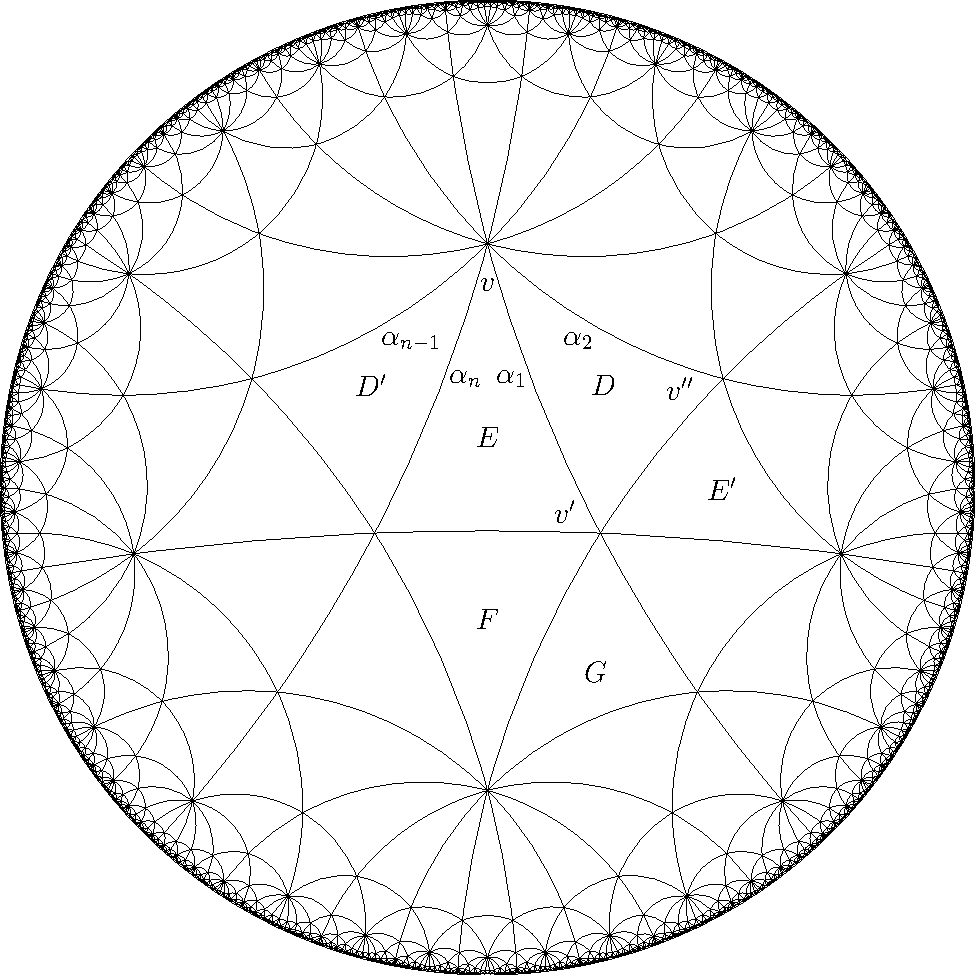
\includegraphics[width=4.5 in]{diagrams/deg33n.pdf}
\end{center}
\end{figure}


	Since $\partial\alpha_1$ separates $D$ and $E,$ we know that $D$ borders $\partial \alpha_2.$ We know that $D$ and $E'$ share two vertices, one of which is $v'.$ The other one cannot be $v$ as the only two chambers which share $v$ and $v'$ are $D,E$ and we assume $E'\neq E.$ Thus we can say that $D,E'$ share two vertices, $v,v''$ and $v''\neq v.$ As before, this means $|\st(v'')|=6.$ Since $D$ borders $\partial \alpha_2$ also know that two vertices of $D$ lie on $\partial \alpha_2.$ The vertex $v'$ cannot lie on $\partial\alpha_2$ as we know that $\partial\alpha_1$ contains $v$ and $v'$ and two distinct walls cannot share two vertices. Therefore, $v''$ lies on $\partial \alpha_2.$ 

	We have that $v''$ is a vertex of $\Sigma$ with $|\st(v'')|=6$ and thus $U_{v''}=U'_{v''}.$ We also know that $E'\in \st(v'')$ and $d(E',C)=d(D,C)-1=d(E,C)=k.$ Thus $d(\proj_{v''}(C),C)\le k.$ By Lemma \ref{lem:deg3fg} this means that $U_{v''}\subset U_k.$ But $\alpha_2$ is a positive root through $v''$ and thus $U_{\alpha_2}\subset U_k$ as desired.

	If $D'\in \st(v')$ from before, then identical arguments show that $U_{\alpha_{n-1}}\subset U_k$ which gives the desired result.
\end{proof}

As we saw in Lemma \ref{lem:generators}, if $\lk(x)$ is associated to $C_2(2)$ or $G_2(3),$ then the inclusion of either $U_2$ or $U_{n-1}$ into $U_k$ will also show that all of $U_v$ is contained in $U_k$ as well. Thus in the setup of this chapter, the previous result is an extension of Lemma \ref{lem:deg3fg}. We are now ready to prove the main result of this section.

\begin{theorem}
	\label{thm:334fg}
	Let $(G,(U_\alpha)_{\alpha\in \Phi},T)$ is an RGD system of type $(W,S)$ satisfying \eqref{assume}. Also assume that $S=\{s,t,u\}$ and $m(s,t)=m(s,u)=3.$ If $\lk(x)$ is the Moufang polygon associated to $C_2(2)$ or $G_2(3),$ where $x$ is the vertex of the fundamental chamber of type $s,$ then $U_+$ is finitely generated.
\end{theorem}
\begin{proof}
	We will show that $U_k\subset U_{k-1}$ for $k\ge 3$ which will show $U_+=U_2$ and thus $U_+$ will be finitely generated by our earlier remarks. Let $k\ge 3$ and choose $\gamma\in \Phi_+$ such that $d(\gamma,C)=k.$ Then we can find a chamber $D$ of $\Sigma$ which borders $\gamma$ such that $d(\gamma,C)=d(D,C)=k.$ Let $D'$ be a chamber adjacent $D$ which is closer to $C,$ or in other words, $d(D',C)=d(D,C)-1.$ Since $D$ borders $\gamma$ we know that $D$ will have two vertices on $\partial \gamma,$ and we also know that $D$ and $D'$ will share two vertices, which means one of the common vertices will also lie on $\partial\gamma.$ Let $v$ be a vertex shared by $D$ and $D'$ which lies on $\partial \gamma.$ By definition, this means $\gamma$ is a positive root at $v$ and thus $U_\gamma\subset U_v.$

	\begin{figure}[h]
	\begin{center}
		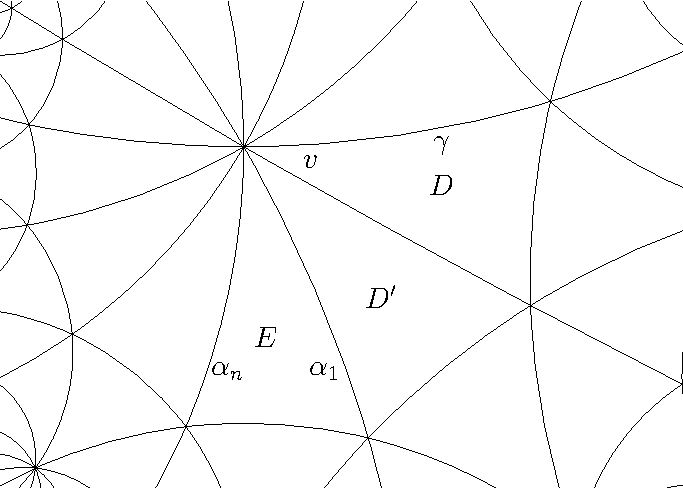
\includegraphics[width=3.5 in]{diagrams/vdef.pdf}
	\end{center}	
	\caption{An example of the chambers $D,D'$ and $E.$}
		\label{fig:vdef}
	\end{figure}

	Let $E=\proj_v(C).$ Then $E$ is the chamber in $\st(v)$ which minimizes the distance to $C.$ Since $D'\in \st(v)$ and $d(D',C)<d(D,C)$ we know that $E\neq D$ and $l=d(E,C)<d(D,C)=k.$ There are exactly two possibilities for $v.$ If $v$ is a vertex of type $t$ or $u$ then $|\st(v)|=6$ and $U_v=U'_v.$ Then we can apply Lemma \ref{lem:deg3fg} to see that $U_v\subset U_l\subset U_{k-1},$ and since $U_\gamma \subset U_v$ we know that $U_\gamma \subset U_{k-1}$ as desired.

	Now suppose that $v$ is a vertex of type $s.$ Then $\lk(v)\cong \lk(x)$ is the Moufang polygon for either $C_2(2)$ or $G_2(3).$ If $d(E,C)\ge 2$ then we can apply Lemma \ref{lem:exdegfg} to say that $U_{\alpha_1},U_{\alpha_n}$ and at least one of $U_{\alpha_2}$ and $U_{\alpha_{n-1}}$ is contained in $U_l\subset U_k.$ Now we can apply Lemma \ref{lem:generators} to see that $U_v\subset U_l\subset U_k.$ Since $\gamma$ is a positive root through $v$ we know that $U_\gamma \subset U_v$ and thus $U_\gamma\subset U_k$ as desired.

	If $d(E,C)<2$ we still have $U_{\alpha_1},U_{\alpha_n}\subset U_l\subset U_2\subset U_{k-1}$ by Lemma \ref{lem:exdegfg} and the assumption that $k\ge 3.$ Let $F,F'$ be the chambers in $\st(v)$ adjacent to $E$ along $\partial\alpha_1$ and $\partial\alpha_n$ respectively. Observation of the local geometry around $v$ shows that $F$ borders $\alpha_2$ and $F'$ borders $\alpha_{n-1}.$ Since $d(F,C)=d(E,C)+1$ we know that $d(\alpha_2,C)\le d(F,C)=d(E,C)+1\le 2.$ This means that $U_{\alpha_2}\subset U_2\subset U_{k-1}$ since $k\ge 3.$ An identical argument shows $U_{\alpha_{n-1}}\subset U_{k-1}$ and thus $U_v\subset U_{k-1}$ by Lemma \ref{lem:generators}. Since $\gamma$ is a positive root through $v$ this also shows that $U_\gamma \subset U_{k-1}$ as desired.

	We have shown for any $k\ge 3$ and positive root $\gamma$ with $d(\gamma,C)=k,$ that $U_\gamma\subset U_{k-1}.$ Since the choice of $\gamma$ was arbitrary we have shown that $U_k\subset U_{k-1},$ and thus by induction we get $U_k=U_2$ for all $k\ge 2.$ By our remarks on $U_k$ this shows that $U_+=U_2$ and thus $U_+$ is finitely generated as desired.
\end{proof}

With this theorem, we have completely determined finite generation for $U_+$ in all RGD systems satisfying \eqref{assume}. In particular, we have determined finite generation for $U_+$ in all rank 3 Kac-Moody groups where the Weyl group $W$ does not have any 2's in the Coxeter diagram. 

Theorem \ref{thm:334fg} shows that in the current setup, not only is $U_+$ finitely generated, but it says that $U_+=U_2$ so that $U_+$ is generated by the root groups $U_\alpha$ with $d(\alpha,C)\le 2.$ There remains the question of whether this generating set is minimal. The answer here is a resounding no, as we will explain. We will not be able to completely solve the question of finding a minimal generating set but we will be able to make a few remarks. First we will pare down the generators of $U_+$ as much as possible by using the commutator relations. While there are similarities between the two cases, it will be easiest to consider each one separately. First suppose that $\lk(x)$ is the group associated to $C_2(2).$ Consider the Coxeter complex of $W$ with the labeling of the roots with $d(\alpha,C)\le 2$ as in Figure \ref{fig:root334}. Of course we do not duplicate roots so every panel does not have a label.

	\begin{figure}[h]
	\begin{center}
		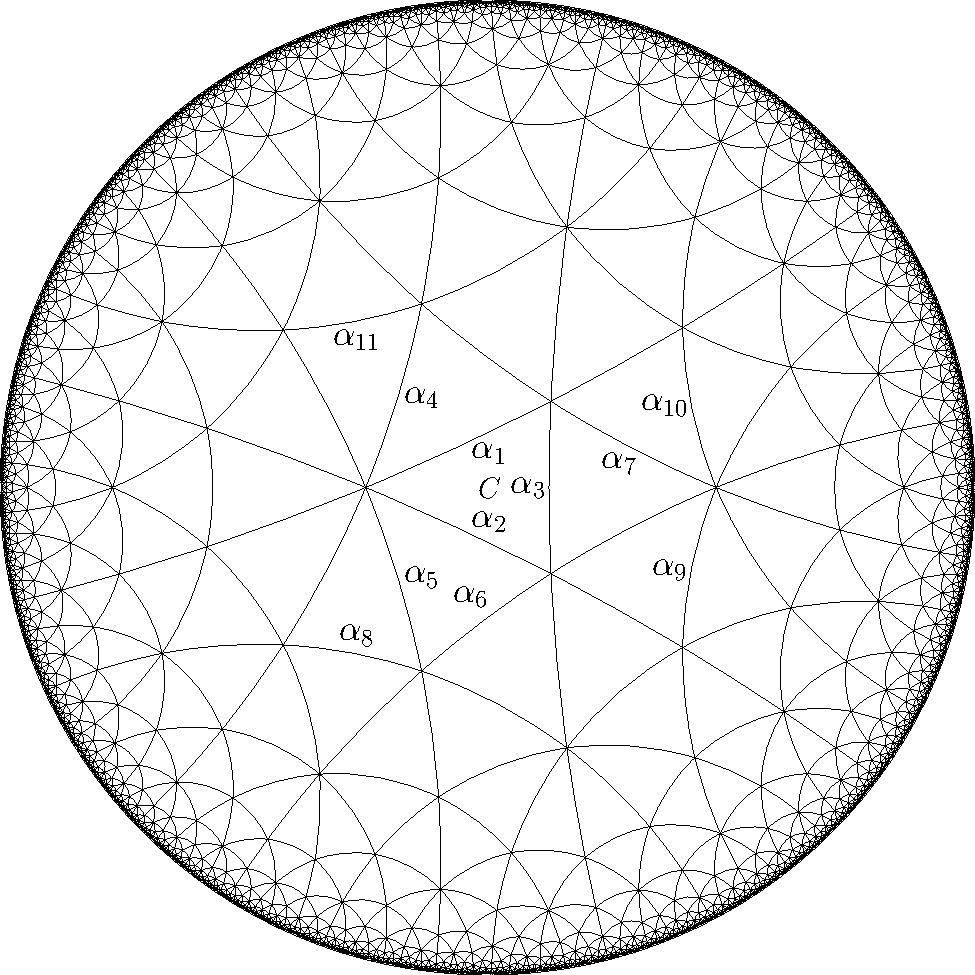
\includegraphics[width=6.5 in]{diagrams/roots334.pdf}
	\end{center}	
	\caption{Unique roots with $d(\alpha,C)\le 2$ with $|\st(x)|=8$}
	\label{fig:root334}
	\end{figure}

Letting $U_i=U_{\alpha_i}$ for all $i,$ we can apply Lemma 3 from \cite{buildings}, as well as Lemma \ref{lem:generators} to write some of these root groups in terms of others. By examining the diagram we get the following relations
\begin{align*}
	U_5&\subset \langle U_1,U_2,U_4\rangle\\
	U_6&\subset \langle U_2,U_3\rangle\\
	U_7&\subset \langle U_1,U_3\rangle\\
	U_8&\subset \langle U_5,U_6\rangle\\
	U_{10}&\subset \langle U_6,U_7,U_9\rangle\\
	U_{11}&\subset \langle U_4,U_7\rangle\\
\end{align*}
all of which together show that $U_+=\langle U_1,U_2,U_3,U_4,U_9\rangle.$


	\begin{figure}[h]
	\begin{center}
		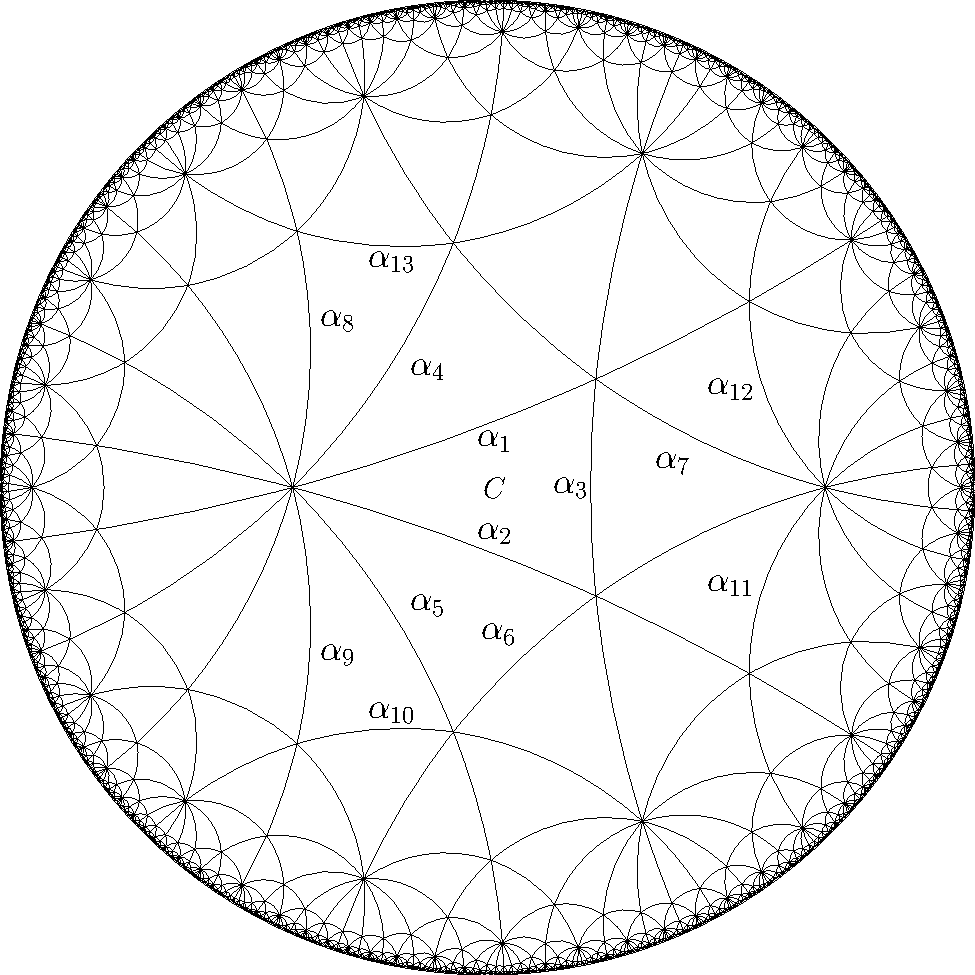
\includegraphics[width=6.5 in]{diagrams/roots336.pdf}
	\end{center}	
	\caption{Unique roots with $d(\alpha,C)\le 2$ with $|\st(x)|=12$}
	\label{fig:root336}
	\end{figure}
Now consider the case when $\lk(x)$ is associated to the group $G_2(3).$ Then we have a similar diagram with labels in Figure \ref{fig:root336}.  Using the same notation as before and similar analysis we get the following relations
\begin{align*}
	U_5,U_8,U_9&\subset \langle U_1,U_2,U_4\rangle\\
	U_6&\subset \langle U_2,U_3\rangle\\
	U_7&\subset \langle U_1,U_3\rangle\\
	U_{10}&\subset \langle U_5,U_6\rangle\\
	U_{12}&\subset \langle U_6,U_7,U_{11}\rangle\\
	U_{13}&\subset \langle U_4,U_7\rangle\\
\end{align*}
which together show that $U_+=\langle U_1,U_2,U_3,U_5,U_{11}\rangle.$ In both of these cases, every group $U_\alpha$ is cyclic of prime order, and thus $U_+$ is actually generated by some choice of generator for each $U_i,$ but this is a minor detail and it is more convenient to work with the root groups as a whole. 

It is possible to make other choices of relations to get other generating sets as well. For example, replacing $U_9$ or $U_{11}$ by $U_{10}$ or $U_{12}$ would also produce a generating set, but one which is more or less equivalent up to some relabeling of the diagram. We will not show that this generating set is minimal but we can make at least one remark.

Any generating set of $U_+$ consisting of root groups must contain at least 3 root groups. If $U_+=\langle U_\alpha,U_\beta\rangle$ then there are 3 possibilities for the pair $\alpha,\beta.$ If $\partial\alpha$ and $\partial\beta$ meet then $\langle U_\alpha,U_\beta\rangle\subset U_v$ where $v$ is the point of intersection. But $U_v$ is finite so this is impossible. If $\alpha$ and $\beta$ are nested the condition \eqref{assume} says that $[U_\alpha,U_\beta]=\{1\}$ so $\langle U_\alpha,U_\beta\rangle=U_\alpha U_\beta$ which is also finite and thus impossible. The last possibility is that the pair $\alpha,\beta$ is not pre-nilpotent. In this case, as stated in \cite{free}, the subgroup $\langle U_\alpha,U_\beta\rangle$ is the free product of $U_\alpha$ and $U_\beta.$ We can always find a root $\gamma$ such that $\alpha\subset \gamma$ and thus $U_\alpha$ and $U_\gamma$ will commute. But the centralizer of $U_\alpha$ in $U_\alpha\ast U_\beta$ is $U_\alpha$ which is a contradiction. Thus any minimal generating set consisting of root groups must contain at least 3 root groups. 

It seems likely based on the commutator relations, and the similarity of these two generating sets that they are in fact minimal generating sets consisting of root groups. There is not much more that can be said at the present time.

\section{Future Questions}
As we have exhausted the question of when groups with RGD systems satisfying \eqref{assume} the next question is how can these assumptions be weakened to get new results. There are 3 main ways that these ideas could continue. The first idea would be to eliminate the restriction that $[U_\alpha,U_\beta]=1$ when $\alpha$ and $\beta$ are nested. This is true for Kac-Moody groups, but is not a consequence of the general RGD axioms, so it is worth considering if we can prove any results without it. Without this assumption, it is still possible to prove groups are finitely generated, but the methods in Chapter \ref{ch:general} would be impossible, as we have no hope of extending $\phi_v$ without this assumption.

The next possibility would be to allow $m(s,t)=2$ in the Weyl group $W.$ This path also leads to difficulties as the triangle condition is an important tool which is lost when $m(s,t)=2.$ Also, preliminary explorations seem to indicate that extending $\phi_v$ is also impossible in the Coxeter complexes which arise in these cases, so once again, a new approach would be needed.

The last area is to allow for $W$ to have higher rank. This seems to have the most promise, and it is even possible that some results about finite generation will follow from the rank 3 case, as there will be subgroups, similar to $U_v,$ for lower dimensional simplices of the building. There are however, two obstacles to face when extending in this manner. This first issue is understanding the geometry of the Coxeter complex $\Sigma.$ For rank 3 Weyl groups, can draw nice 2 dimensional pictures to get an Idea of what is happening in $\Sigma.$ A large help was the code seen in the appendix which allowed me to nicely draw Coxeter complexes for rank 3 $W.$ There is some though of writing similar code to possibly 3D print models of the Coxeter complex for rank 4 Weyl groups, which could potentially be helpful.

The other problem, but perhaps the most manageable, is that for higher rank, the Coxeter complex may not live so nicely as a model of hyperbolic space. It does seem that the group theoretic methods described in Chapter \ref{ch:general} will translate however, and it seems promising that something can be said for at least rank 4 cases as well.



\end{document}
